\documentclass{llncs}


% \usepackage[T1]{fontenc}
\usepackage[utf8]{inputenc}
\usepackage{microtype}
%\usepackage[numbers]{natbib}
\usepackage{xspace}
\usepackage{balance}
\usepackage{hyperref}
\usepackage{url}
\usepackage{breakurl}
\usepackage{enumerate}
\usepackage{enumitem}

\usepackage{listings}
\lstdefinelanguage{program}{%
  keywords={%
    let,pass,function,%
    var,const,bool,int,void,atomic,%
    while,do,if,then,else,assume,assert,call,return,rule,forall,with,new,choose,skip,%
    task,async,yield,for,wait%
  },
  morecomment=[l]{//},
  morecomment=[s]{/*}{*/},
  morecomment=[n]{(*}{*)},
  mathescape=true,
  escapeinside=`',
}
\lstset{
  language={program},
  basicstyle=\ttfamily\scriptsize
}


\usepackage{multirow}

\usepackage{graphicx}
\usepackage{tikz}
\usetikzlibrary{positioning,shapes,shadows,arrows}
\usetikzlibrary{decorations.pathmorphing,snakes}
\usepackage{tkz-graph}
\usepackage{moresize}

%\newenvironment{proof}{\paragraph{Proof.}}{\hfill$\square$}

\def\ttat{\mitt{@}} % the at package clobbers this
\usepackage{at}

%\usepackage{amsthm}
\usepackage{amsmath}
\usepackage{amsfonts}
\usepackage{amssymb}
\usepackage{latexsym}
\usepackage{wasysym} % causing problems with llncs's bold vectors
\usepackage{stmaryrd}
\usepackage{alltt}
\usepackage{mathpartir}
\usepackage[ligature,reserved,inference]{semantic}
\usepackage[lined]{algorithm2e}
\usepackage{graphicx}
\usepackage{pgf}
\usepackage{tikz}
\usepackage{multicol}
\usepackage{fancyvrb}
\usepackage{rotating}
\usepackage{latexsym}
\usepackage{tabulary}
\usepackage{wrapfig}
\usepackage{caption,subcaption}
%\usepackage{pslatex}

\usetikzlibrary{arrows,automata}
\usetikzlibrary{positioning,shapes,shadows}
\usetikzlibrary{decorations}
\makeatletter

%% Macros plus
\input macros
%\input macros-programs
\input macros-local

\newcommand{\todo}[1]{\textcolor{blue}{[TODO: #1]}}
\newcommand{\shuvendu}[1]{\textcolor{green}{[SKL: #1]}}
\newcommand{\send}[2]{\mathrm{send}_{#1}({#2})}
\newcommand{\rec}[2]{\mathrm{rec}_{#1}({#2})}

\newcommand{\senda}[1]{\mathrm{send}({#1})}
\newcommand{\reca}[1]{\mathrm{rec}({#1})}
\newcommand{\paral}{\,||\,}


\newcommand{\asynch}[1]{\mathrm{Asynch}\text{-}\mathrm{#1}}
\newcommand{\synch}[1]{\mathrm{Synch}\text{-}\mathrm{#1}}
\newcommand\asynchTr[1]{\mathrm{asTr}({#1})} %{  \llbracket {#1} \rrbracket_{asynch} }
\newcommand\asynchExec[1]{\mathrm{asEx}({#1})} %{  \llbracket {#1} \rrbracket_{asynch} }
\newcommand\synchTr[2]{\mathrm{sTr}_{#2}({#1})} %{  \llbracket {#1} \rrbracket_{asynch} }
\newcommand\synchExec[2]{\mathrm{sEx}_{#2}({#1})} %{  \llbracket {#1} \rrbracket_{asynch} }
\newcommand{\xRightarrow}[2][]{\ext@arrow 0359\Rightarrowfill@{#1}{#2}}

\newcommand\asynchSt[1]{\mathrm{asSt}({#1})} %{  \llbracket {#1} \rrbracket_{asynch} }
\newcommand\synchSt[2]{\mathrm{sSt}_{#2}({#1})} %{  \llbracket {#1} \rrbracket_{asynch} }

\author{}
\institute{}

\title{On the Completeness of Verifying Message Passing Programs under Bounded Asynchrony}
%Getting Rid of Unbounded Buffers in the Verification of Message Passing Systems} %% [Short Title] is optional;



                                        %% when present, will be used in
                                        %% header instead of Full Title.
%\titlenote{with title note}             %% \titlenote is optional;
                                        %% can be repeated if necessary;
                                        %% contents suppressed with 'anonymous'
%\subtitle{Subtitle}                     %% \subtitle is optional
%\subtitlenote{with subtitle note}       %% \subtitlenote is optional;
                                        %% can be repeated if necessary;
                                        %% contents suppressed with 'anonymous'



%% Author information
%% Contents and number of authors suppressed with 'anonymous'.
%% Each author should be introduced by \author, followed by
%% \authornote (optional), \orcid (optional), \affiliation, and
%% \email.
%% An author may have multiple affiliations and/or emails; repeat the
%% appropriate command.
%% Many elements are not rendered, but should be provided for metadata
%% extraction tools.

%%% Author with single affiliation.
%\author{First1 Last1}
%\authornote{with author1 note}          %% \authornote is optional;
%                                        %% can be repeated if necessary
%\orcid{nnnn-nnnn-nnnn-nnnn}             %% \orcid is optional
%\affiliation{
%  \position{Position1}
%  \department{Department1}              %% \department is recommended
%  \institution{Institution1}            %% \institution is required
%  \streetaddress{Street1 Address1}
%  \city{City1}
%  \state{State1}
%  \postcode{Post-Code1}
%  \country{Country1}
%}
%\email{first1.last1@inst1.edu}          %% \email is recommended
%
%%% Author with two affiliations and emails.
%\author{First2 Last2}
%\authornote{with author2 note}          %% \authornote is optional;
%                                        %% can be repeated if necessary
%\orcid{nnnn-nnnn-nnnn-nnnn}             %% \orcid is optional
%\affiliation{
%  \position{Position2a}
%  \department{Department2a}             %% \department is recommended
%  \institution{Institution2a}           %% \institution is required
%  \streetaddress{Street2a Address2a}
%  \city{City2a}
%  \state{State2a}
%  \postcode{Post-Code2a}
%  \country{Country2a}
%}
%\email{first2.last2@inst2a.com}         %% \email is recommended
%\affiliation{
%  \position{Position2b}
%  \department{Department2b}             %% \department is recommended
%  \institution{Institution2b}           %% \institution is required
%  \streetaddress{Street3b Address2b}
%  \city{City2b}
%  \state{State2b}
%  \postcode{Post-Code2b}
%  \country{Country2b}
%}
%\email{first2.last2@inst2b.org}         %% \email is recommended

\begin{document}

\pagestyle{headings}
\bibliographystyle{splncs03}


%% Paper note
%% The \thanks command may be used to create a "paper note" ---
%% similar to a title note or an author note, but not explicitly
%% associated with a particular element.  It will appear immediately
%% above the permission/copyright statement.
%\thanks{with paper note}                %% \thanks is optional
                                        %% can be repeated if necesary
                                        %% contents suppressed with 'anonymous'


%% Abstract %%%%%%%%%%%%%%%%%%%%%%%%%%%%%%%%%%%%%%%%%%%%%

%% Abstract
%% Note: \begin{abstract}...\end{abstract} environment must come
%% before \maketitle command


\maketitle

\begin{abstract}
We address the problem of verifying message passing programs, defined as a set of parallel processes communicating through unbounded FIFO buffers.
%Their verification is hard, undecidable in general. An important issue is the design of verification methods that explore subsets of the asynchronous behaviors of the program in order to draw useful conclusions about its correctness. 
%Existing approaches in this line of research are either not applicable to systems with unbounded buffers, or restricted in scope, or highly complex, or not guaranteed to terminate, or are based on approximate analyses without guarantees of completeness. In this paper 
We introduce a bounded analysis that explores a special type of computations, called $k$-synchronous. These computations can be viewed as (unbounded) sequences of interaction phases, each phase allowing at most $k$ send actions (by different processes), followed by a sequence of receives corresponding to sends in the same phase. We give a procedure for deciding {\em $k$-synchronizability} of a message passing program, i.e., whether every computation is equivalent (has the same happens-before relation) to one of its $k$-synchronous computations. We also show that 
%This procedure consists in checking a reachability property on the $k$-synchronous computations of an instrumented version of the program (it doesn't have to deal with arbitrary asynchronous computations). We show that 
reachability over $k$-synchronous computations and checking $k$-synchronizability are both PSPACE-complete. Furthermore, we introduce a class of programs called {\em flow-bounded} for which the problem of deciding whether there exists a $k>0$ for which the program is $k$-synchronizable, is decidable.
%
% is decidable and PSPACE-complete. T
%
%of them being a sequence of at most $K$ sends (by different processes), followed by a sequence of receives corresponding to sends in the same phase.
%
%We propose an approach for the verification of message passing programs that avoids manipulating explicitly unbounded buffers, and for which it is possible to ensure completeness for a wide and practically relevant class of programs. 
%
%
%
%The contribution of this paper are:
%
%\begin{itemize}
%
%\item A new bounded analysis for message passing programs called Exchange Bounded Analysis (EBA), based on exploring a special type of computations called $K$-synchronous, for a given integer $K>0$. Such computations are successions of interaction phases, each of them being a sequence of at most $K$ sends (by different processes), followed by a sequence of receives corresponding to sends in the same phase. The complexity of state reachability under EBA is PSPACE-complete.
%
%\item A procedure for deciding {\em $K$-synchronizability} of a message passing programs, i.e., for given program, determine whether every  computation of that program is equivalent (has the same happen-before relation) to one of its $K$-synchronous computations. Importantly, the decision procedure never consider the asynchronous semantics (with unbounded buffers); it is based on an exchange-bounded analysis of an instrumented version of the original program. Consequently, the state reachability problem is decidable for $K$-synchronizable programs, and deciding both $K$-synchronizability and state reachability in this case is PSPACE-complete.
%
%\item A procedure for deciding {\em synchronizability}, for a class of message passing programs called {\em flow-bounded programs}, i.e., for a given program in this class, determine whether there exists a $K>0$ for which the program is $K$-synchronizable. The decision procedure uses an iteration of exchange bounded analyses of instrumented versions of the program. Consequently, the state reachability problem is decidable for synchronizable flow-bounded programs.
%%Deciding  synchronizability and state reachability in this case is PSPACE-complete. NOOONNNNNNNN
%
%\item Our approach is also applicable to verifying the existence of deadlocks.
%
%\end{itemize}
%
%All programs we have encountered in practice are synchronizable, and they are either in the syntactical class of flow-bounded programs, or they are outside this class but still synchronizable for a bound $K$ that is easy to find.
\end{abstract}

%% ACM Stuff %%%%%%%%%%%%%%%%%%%%%%%%%%%%%%%%%%%%%%%%%%%%%




%% Paper body %%%%%%%%%%%%%%%%%%%%%%%%%%%%%%%%%%%%%%%%%%%%%

\input intro
\input overview
\input asynch-semantics
\input synch-semantics
\input robustness
\input verification
\input decidability
\input related
%\input conclusions

\clearpage

%\bibliographystyle{plain}
\bibliography{references}

\newpage
\appendix
%!TEX root = main.tex
\section{Motivating Examples}\label{asec:motivation}

\begin{figure}[t]
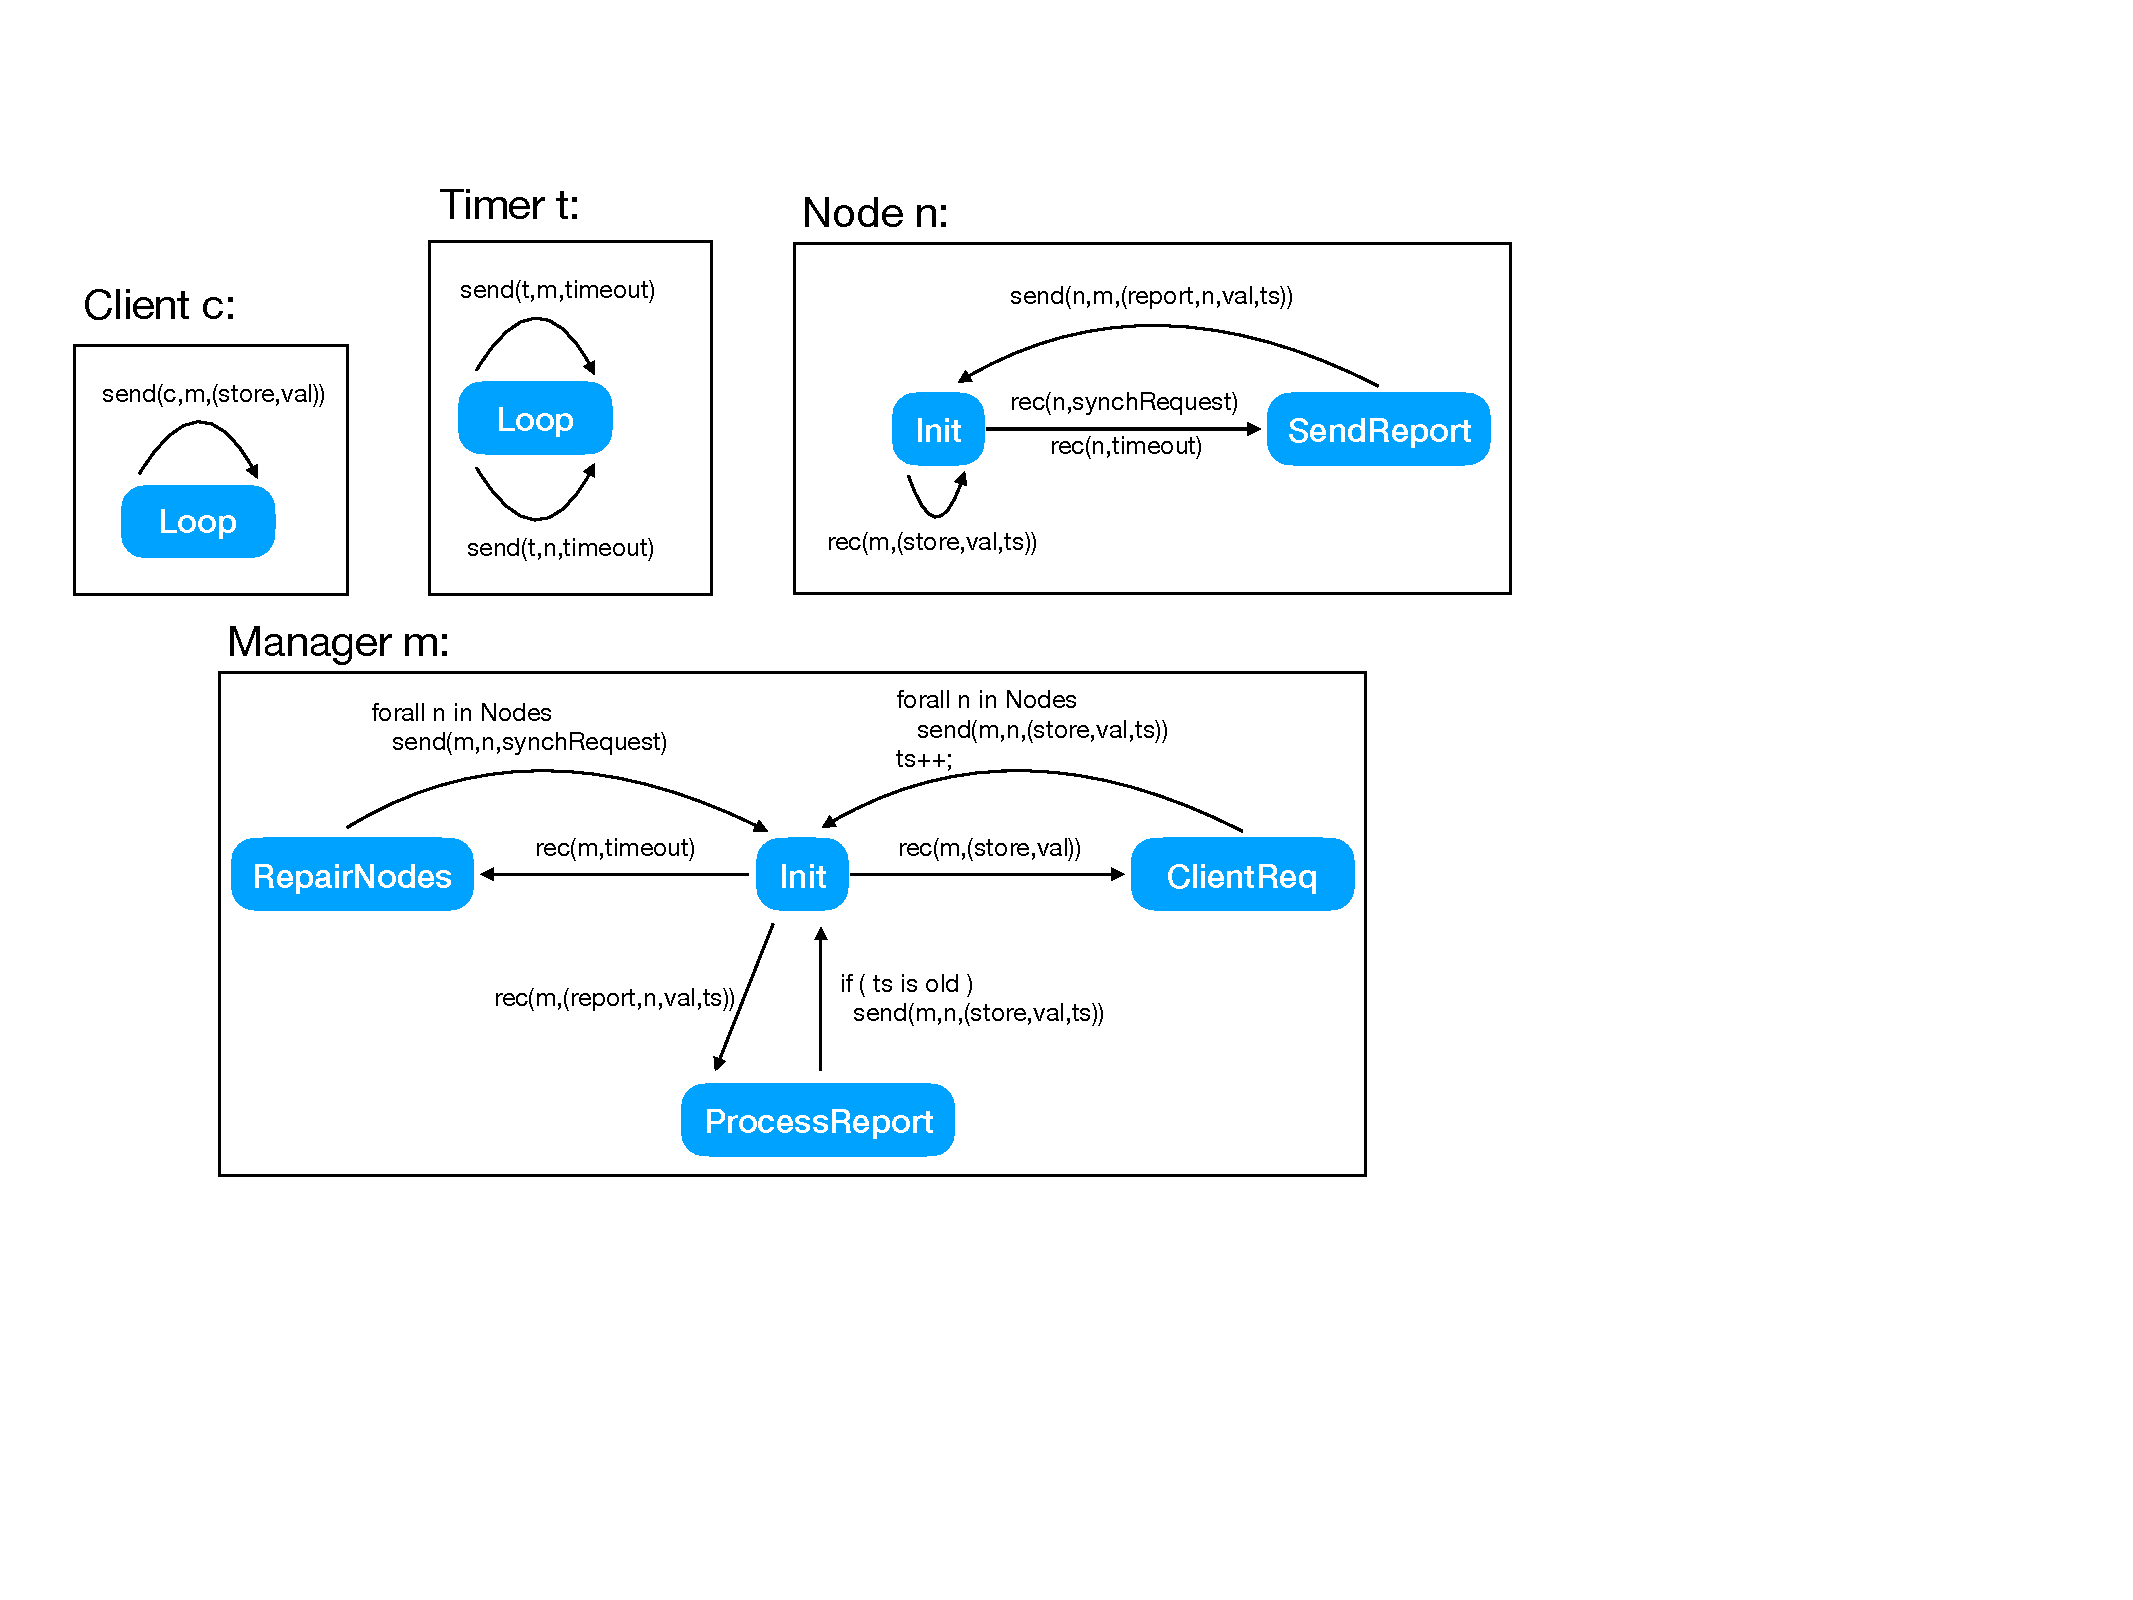
\includegraphics[width=10cm]{replication.pdf}
\caption{A replication storage protocol.}
\label{fig:replication}
\end{figure}

\begin{figure}[t]
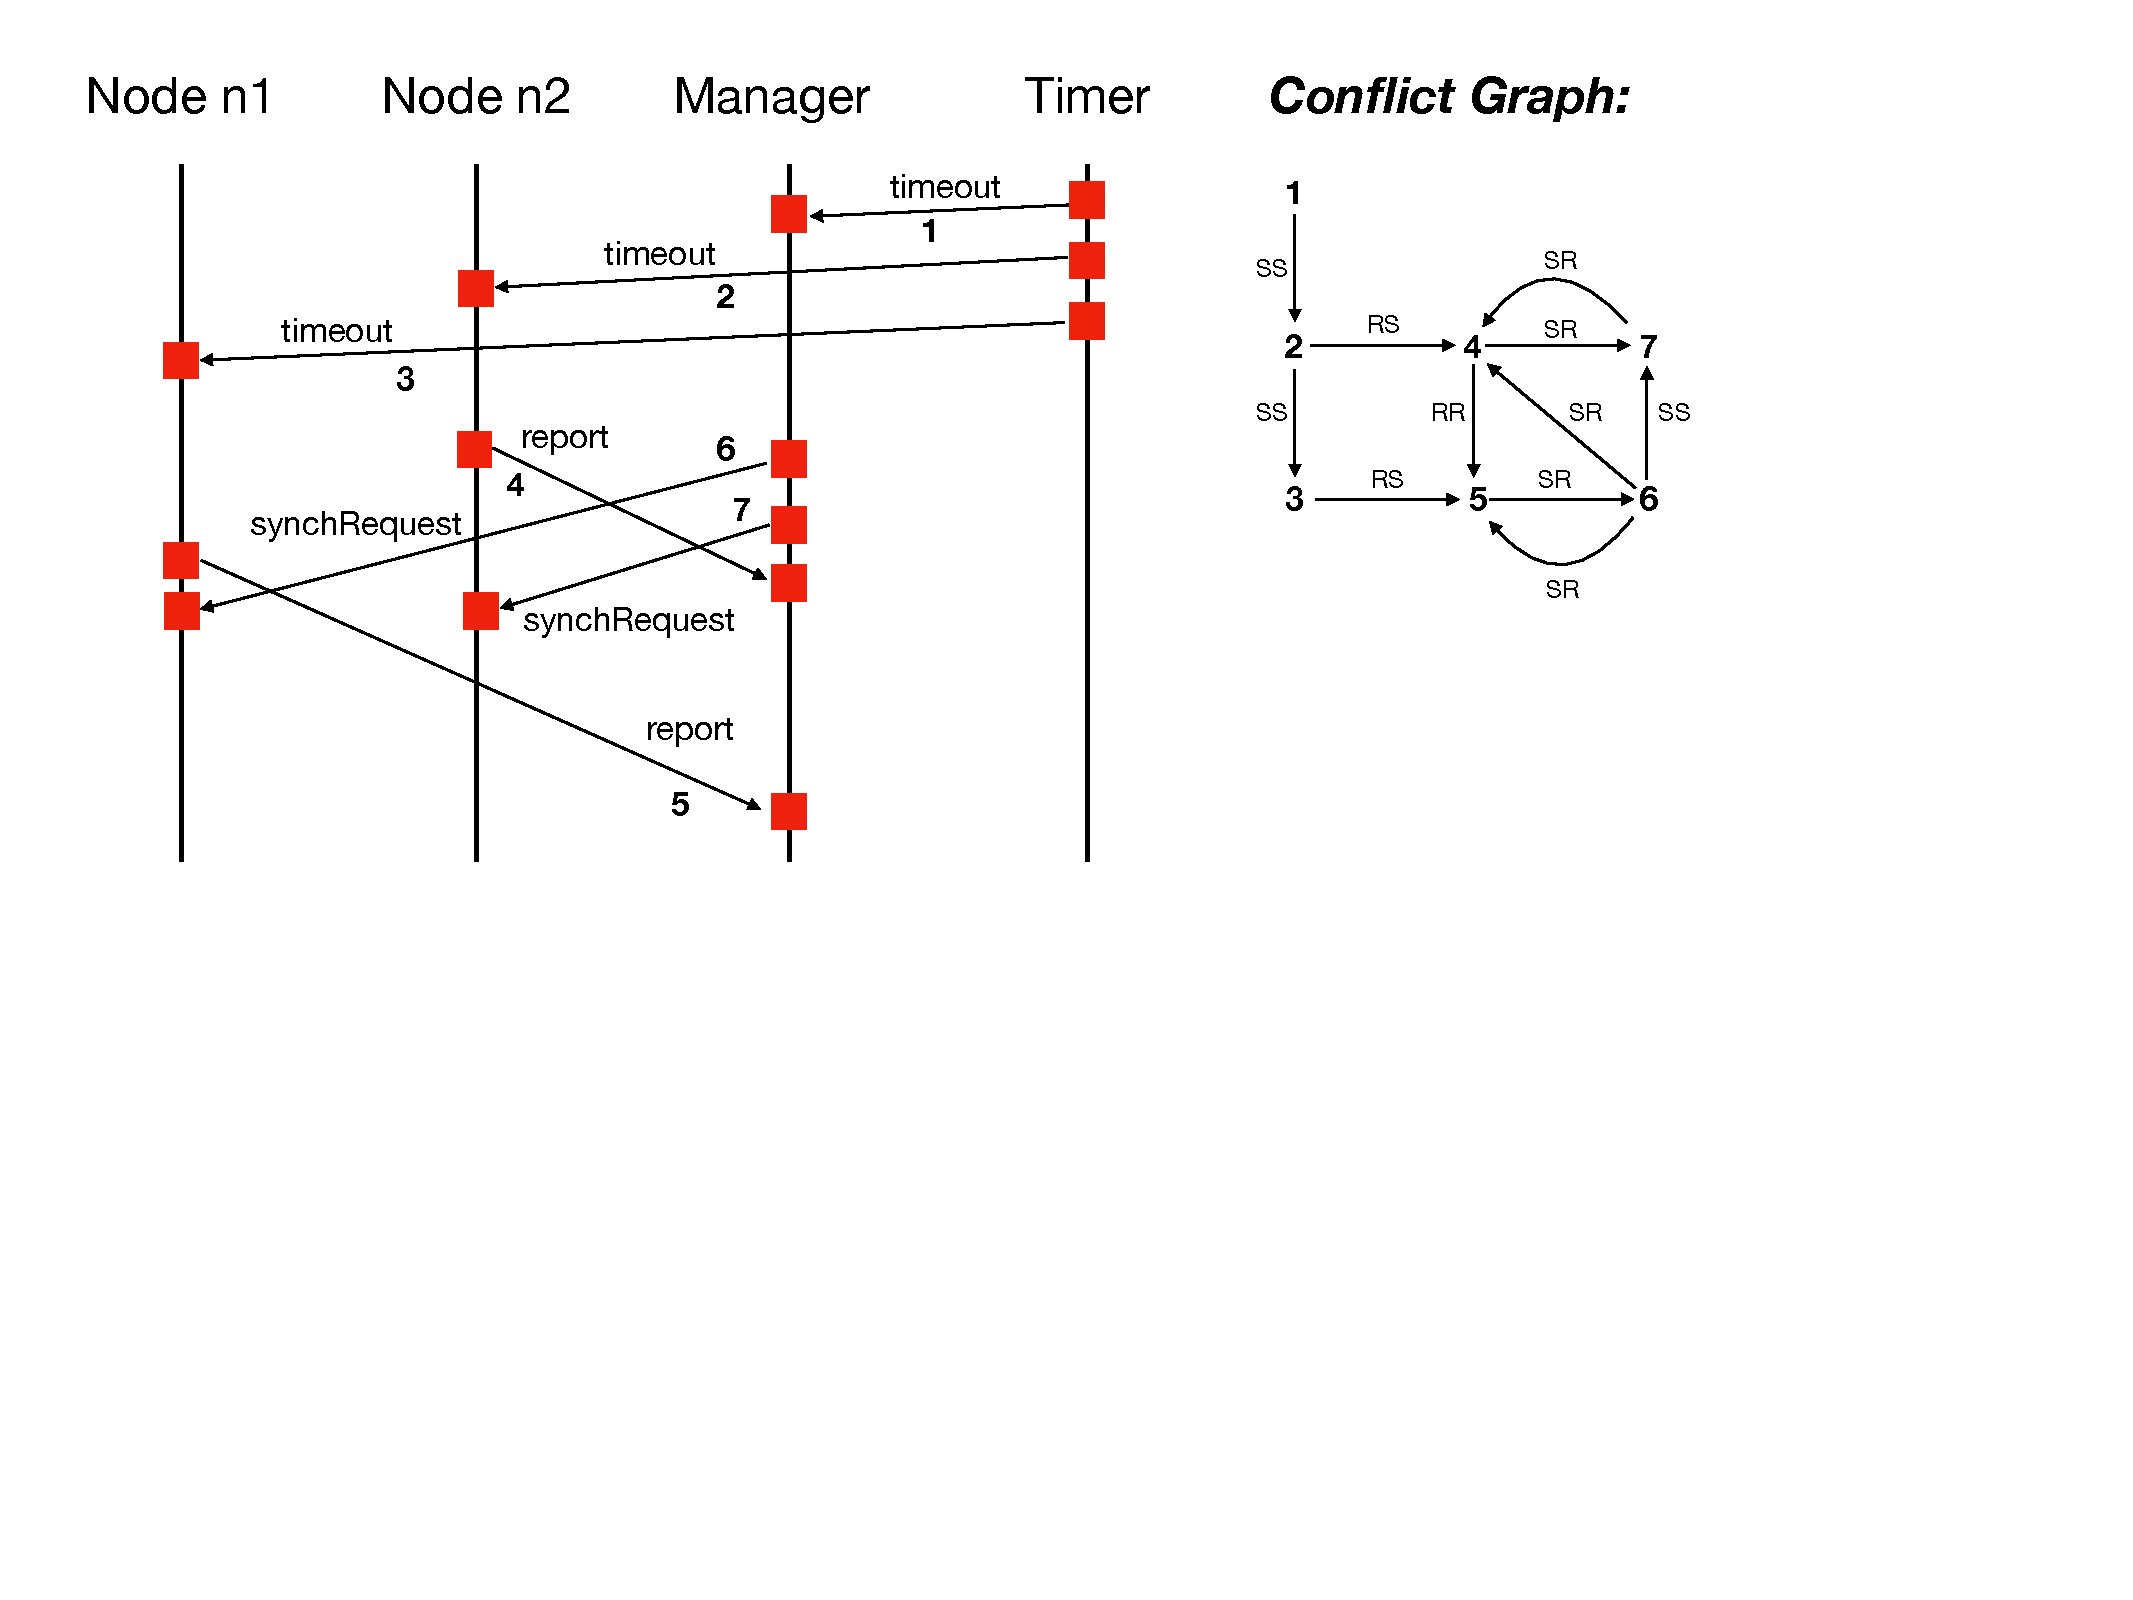
\includegraphics[width=7cm]{MSC-storage.pdf}
\caption{An execution of the replication storage protocol and its conflict graph.}
\label{fig:replic-exec}
\end{figure}


We present an example illustrating the fact that exchanges can involve not only 2 processes but several ones, maybe all the processes of a system. Figure \ref{fig:replication} shows a replication storage protocol. A client can send update requests to the manager who is in charge of maintaining several storage replicas on different nodes. When the manager receives an update request from the client, it forwards this message to all the nodes. However, since messages can be delayed, the information in the nodes can be different at various points in time. Then, a mechanism is used to force regularly synchronization between the data versions stored in the different nodes. This mechanism is based on (1) using time-stamps for each message that is sent  by the manager to the nodes, and (2) a timer that triggers synchronizations: the timer can send timeout messages to either the manager or to the nodes. When a node receives such a timeout message, it sends a report to the manager with its current data value, and when the manager receives the timeout message, it sends to all nodes a message requesting a synchronization. When a node receives the synchronization request, it sends to the manager a report with its last value. After each reception of a report from a node, the manager checks if the received value is up-to-date using its time-stamp, and if not, it sends the most recent value to the node. Now, since the nodes and the manager may all receive timeout messages from the timer, nodes can start sending reports to the manager while the latter is already sending them synchronization requests. This leads to an exchange that may involve all the nodes, in addition to the manager. This situation is shown in Figure \ref{fig:replic-exec}. The conflict graph shown on the right of the figure contains a cycle of size 4, which is in this case the number of involved processes (two nodes and one manager), plus 1, which means that the considered computation is not 3-synchronizable. It can be checked that the system is actually 4-synchronizable. 

\section{Asynchronous Semantics of Message Passing Systems}\label{asec:semantics}

Formally, configuration $c=\tup{\vec{l},\vec{b}}$ is a vector  $\vec{l}$  of local states together with a vector $\vec{b}$ of message buffers  that are
represented as sequences of message payloads tagged with unique identifiers. The identifiers are used only for technical reasons, to identify a ``matching'' relation
between sends and receives.  These two vectors are indexed by elements of $\<Pids>$.
For a vector $\vec{x}$, let $\vec{x}_p$ denote the element of $\vec{x}$ of index $p$.
%The state of the process $p$ is defined by the local state $\vec{l}_p$ and the message buffer $\vec{b}_p$.
The initial configuration $c_0$ of the system $\mathcal{S}$ is the tuple of initial local states together with empty message buffers, i.e., 
$c_0=\tup{\vec{l},\vec{b}}$ where $\vec{l}_p=l_p^0$ and $\vec{b}=\epsilon$ for each $p\in\<Pids>$.
%The set of configurations is denoted by $C$.

\begin{figure} [t]
\footnotesize{
  \centering
  \begin{mathpar}
    \inferrule[send]{
      m= (i,v) \\ 
      i\in \<Mids>\mbox{ fresh} \\
      (\vec{l}_p,\senda{p,q,v},l)\in \delta_p 
    }{
      \vec{l},\vec{b}
      \xrightarrow{\send{i}{p,q,v}}
      \vec{l}[\vec{l}_p\gets l],\vec{b}[\vec{b}_q\gets \vec{b}_q\cdot m]
    }%\hspace{5mm}
    
    \inferrule[receive]{
      \vec{b}_q = (i,v) \cdot b \\
      (\vec{l}_q,\reca{q,v},l)\in \delta_q
    }{
      \vec{l},\vec{b}
      \xrightarrow{\rec{i}{q,v}}
      \vec{l}[\vec{l}_q\gets l],\vec{b}[\vec{b}_q\gets b]
    }%\hspace{5mm}
    
%    \inferrule[local]{ 
%      l\in \delta(\vec{l}_p,\epsilon) \neq \emptyset
%    }{
%      \vec{l},\vec{b}
%      \xrightarrow{\epsilon}
%      \vec{l}[\vec{l}_p\gets l],\vec{b}
%    }%\hspace{5mm}
  \end{mathpar}
  }
% \vspace{-5mm}
  \caption{The asynchronous semantics of a message passing system $\mathcal{S}$. For a vector $\vec{x}$, $\vec{x}[\vec{x}_p\gets E]$ is the vector $\vec{y}$ with $\vec{y}_q=\vec{x}_q$, for every $q\neq p$, and $\vec{x}_p=E$. Also, $\cdot$ denotes the concatenation of two sequences.
  %$\vec{b}[\vec{b}_q.\ \mathrm{add}(m)]$ denotes the vector of message buffers obtained from $\vec{b}$ by calling the method $\mathrm{add}(m)$ of the element of index $q$.
  }
  \label{fig:asynch-sem}
%\vspace{-6mm}
\end{figure}

The transition relation $\rightarrow$ in Figure~\ref{fig:asynch-sem} is determined by a message passing system $\mathcal{S}$, and maps
a configuration $c_1$ to another configuration $c_2$ and indexed action $a\in S_{id}\cup R_{id}$.
The effect of a \textsc{send} transition is to enqueue the message payload tagged with a fresh identifier to the buffer of the destination, and the effect of a \textsc{receive} transition is to dequeue a message from the local buffer.

An \emph{execution} of a system $\mathcal{S}$ under the asynchronous semantics to configuration ${c}_n$
is a sequence of indexed actions $a_1 \ldots a_n$ such that 
there exists a configuration sequence ${c}_0 {c}_1 \ldots {c}_n$ with
%\vspace{-2mm}
%\begin{align*}
$  {c}_m \xrightarrow{a_{m+1}} {c}_{m+1}$
%\end{align*}
%%\vspace{-1.5mm}
%\noindent
for all $0 \le m < n$. 
We 
%call the sequence $a_1 \ldots a_n$ the \emph{log} of ${c}_0 {c}_1 \ldots
%{c}_n$ and we 
say that ${c}_n$ is reachable in $\mathcal{S}$ under the asynchronous semantics. % with log $a_1\ldots a_n$. 
The \emph{reachable local state vectors} of $\mathcal{S}$, denoted by $\asynchSt{\mathcal{S}}$, is the
set of local state vectors in reachable configurations.
%
The set of executions of $\mathcal{S}$ under the asynchronous semantics is denoted by $\asynchExec{\mathcal{S}}$.
In the following, we don't distinguish between executions obtained by a consistent renaming of the message identifiers. 



\section{Detecting deadlocks}\label{asec:deadlocks}

In addition to assertion/invariant checking, we show that the problem of detecting deadlocks in a $k$-synchronizable system can also be solved using the $k$-synchronous semantics instead of the asynchronous one. For a process $p$, a state $l\in \<Lsts>_p$ is called \emph{receiving} when $(l,a,l')\in\delta_p$, for some $l'$, implies that $a\in R_p$. For instance, the state {\tt Init} of the process {\tt Manager} in Figure~\ref{fig:commit} is receiving. The state $l$ is called \emph{final} when there exists no $l'$ and $a$ such that $(l,a,l')\in\delta_p$.

We consider several notions of deadlock: a configuration $c=(\vec{l},\vec{b})$ is called 
\begin{itemize}
	\item \emph{empty-buffer deadlock} when all the buffers are empty, there exists at least one process waiting for a message, and all the other processes are either in a final or receiving state, i.e., $\vec{b}=\vec{\epsilon}$, there exists $p\in\<Pids>$ such that $(\vec{l}_p,r,l')\in\delta_p$ for some $r\in R$, and for all $q\in \<Pids>$, $\vec{l}_q$ is receiving or final,
	\item \emph{orphan message configuration} when there is at least a non-empty buffer and each process is in a final state, i.e., $\vec{b}\neq\vec{\epsilon}$ and for all $p\in \<Pids>$, $\vec{l}_p$ is final,
	\item \emph{unspecified reception} when some process is prevented from receiving any message from its buffer, i.e., there exists $p\in\<Pids>$ such that $\vec{l}_p$ is receiving, and for all $\reca{p,v}\in R$, if $(\vec{l}_p,\reca{p,v},l')\in \delta_p$, for some $l'$, then $\vec{b}_p\not\in v\<Val>^*$.
\end{itemize}

We show that reachability of such configurations in the original asynchronous semantics can be reduced to reachability problems over the synchronous semantics, provided that the system is $k$-synchronizable. The constraints over the buffers of the asynchronous configurations are replaced by constraints over the executions (traces) of the synchronous semantics. For instance, an execution reaching an empty-buffer configuration is ``equivalent'' to a synchronous \emph{matched} execution where every sent message has been received (assuming $k$-synchronizability).

We extend the notion of empty-buffer deadlock to configurations of the synchronous semantics by removing the condition that the buffers are empty.

\begin{theorem}\label{th:deadlock1}
A $k$-synchronizable system $\mathcal{S}$ reaches an empty-buffer deadlock configuration under the asynchronous semantics iff the $k$-synchronous semantics of $\mathcal{S}$ admits a matched execution to an empty-buffer deadlock configuration.
\end{theorem}
\begin{proof}
We prove the only-if direction, the reverse being similar. 
Let $e$ be an execution in $\asynchExec{\mathcal{S}}$ to an empty-buffer deadlock configuration $(\vec{l},\vec{\epsilon})$. Since the buffers are empty, by the definition of the asynchronous semantics, we get that $e$ is matched. By $k$-synchronizability, there exists a permutation $e'$ of $e$ that belongs to $\synchExec{\mathcal{S}}{k}$. Then, by Lemma~\ref{lem:undist}, $e'$ is an execution to a configuration $(\vec{l},B)$, for some $B$, which finishes the proof.
\end{proof}

A configuration $(\vec{l},B)$ of the synchronous semantics is called \emph{final} when every local state $\vec{l}_p$ with $p\in\<Pids>$ is final. The proof of the following result is similar to that of Theorem~\ref{th:deadlock1}, the only addition being that an asynchronous execution to a configuration with non-empty buffers corresponds to a synchronous execution with unmatched send actions (provided that the system is $k$-synchronizable). 

\begin{theorem}
A $k$-synchronizable system $\mathcal{S}$ reaches an orphan message configuration under the asynchronous semantics iff the $k$-synchronous semantics of $\mathcal{S}$ admits an execution containing at least one unmatched send to a final configuration.
\end{theorem}

%Let $(\vec{l},B)\xRightarrow{e}{_k} (\vec{l'},B')$ be a \textsc{$k$-exchange} transition. This transition is called \emph{$p$-blocked} when intuitively, $p$ is in a receiving state but it can't receive any message sent to $p$ in $e$, i.e., $\vec{l}_p$ is receiving, $e$ contains an unmatched send action $s$ with destination $p$ and there exists no extension of $e$ by adding a receive $r$ matching $s$ (and possibly other actions) such that $(\vec{l},B)\xRightarrow{e'}{_k} (\vec{l''},B'')$ is valid, for some $(\vec{l''},B'')$.

A local state $l$ of a process $p$ is called \emph{$V$-receiving} when it is receiving and the set of messages that can be received in $l$ is exactly $V$, i.e., for all $v$,  $v\in V$ iff there exists $l'\in \<Lsts>_p$ such that $(l,\reca{p,v},l')\in \delta_p$. A configuration $(\vec{l},B)$ of the synchronous semantics is called \emph{$(p,V)$-receiving} when $\vec{l}_p$ is $V$-receiving. 
Given an execution $e$, let $\mathit{minUnmatched}(e,p)$ be the set of unmatched send actions in $e$ which are minimal in the causal relation of $tr(e)$ among unmatched send actions with destination $p$, i.e., $\mathit{minUnmatched}(e,p)$ is the set of unmatched send actions $\send{i}{p',p,v}$ in $e$ such that for every other unmatched send action $\send{j}{p'',p,v}$ in $e$ we have that $\send{i}{p'',p,v}\not\leadsto_{tr(e)}\send{i}{p',p,v}$.

\begin{theorem}
A $k$-synchronizable system $\mathcal{S}$ reaches an unspecified reception configuration under the asynchronous semantics iff there exists some $p\in \<Pids>$ such that the $k$-synchronous semantics of $\mathcal{S}$ admits an execution $e$ to a $(p,V)$-receiving state and 
\begin{align*}
\{v: \exists \send{i}{p',p,v}\in \mathit{minUnmatched}(e,p)\}\setminus V \neq \emptyset.
\end{align*}
\end{theorem}
\begin{proof}
For the only-if direction, let $e$ be an execution in $\asynchExec{\mathcal{S}}$ to an unspecified reception configuration $(\vec{l},\vec{b})$. Then, there exists $p\in\<Pids>$ such that $\vec{l}_p$ is $V$-receiving, for some $V\in\<Vals>$, and $v_p\not\in V$, where $v_p$ is the head of $\vec{b}_p$ (the first message to be dequeued). Therefore, $e$ contains an unmatched send action $\send{i}{p',p,v_p}$ which is also the first among unmatched send actions with destination $p$ (otherwise, $v_p$ would not be the first message in the buffer of $p$). Therefore, $\send{i}{p',p,v_p}\in \mathit{minUnmatched}(e,p)$. By $k$-synchronizability, there exists a permutation $e'$ of $e$ that belongs to $\synchExec{\mathcal{S}}{k}$. By Lemma~\ref{lem:undist}, $e'$ is an execution to a configuration $(\vec{l},B)$, for some $B$, which is $(p,V)$-receiving. Since $e$ and $e'$ have the same trace, we get that $\send{i}{p',p,v_p}\in \mathit{minUnmatched}(e',p)$ as well, which finishes the proof of this direction.

For the if direction, assume that the $k$-synchronous semantics of $\mathcal{S}$ admits an execution $e$ as above. Let $\send{i}{p',p,v}$ be an action in $\mathit{minUnmatched}(e,p)$ such that $v\not\in V$. Because $\send{i}{p',p,v}$ is minimal among unmatched send actions with destination $p$, there exists a permutation $e'$ of $e$ where it is the first unmatched send with destination $p$. As a direct consequence of the definitions, we get that $e$ is an execution to an unspecified reception configuration.
\end{proof}

\section{Proofs of Section~\ref{sec:characterizations}}\label{asec:characterizations}

\begin{theorem}\label{lem:cg_k}
A trace $t$ satisfying causal delivery is $k$-synchronous if{f} every cycle in its conflict-graph is good and of size at most $k$.
\end{theorem}
\begin{proof}
For the only if direction, $t$ is the trace of an execution $e\in \synchExec{\mathcal{S}}{k}$ for some system $\mathcal{S}$. The execution $e$ is obtained through a sequence of \textsc{$k$-exchange} transitions. The set of actions of every node $v$ of $CG_t$ appear in the label of a single such transition. Moreover, for every cycle in $CG_t$, the actions corresponding to the nodes in this cycle occur in the label of a single \textsc{$k$-exchange} transition. Therefore, every cycle in $CG_t$ is good and of size at most $k$.

For the if direction, we first show that any strongly-connected component $C$ of $CG_t$ is $k$-synchronous. Since all the cycles in $CG_t$ are of size at most $k$, we get that $C$ contains at most $k$ nodes. The case of strongly-connected components formed of a single node $v$ is trivial. The actions corresponding to $v$ are either a matching pair of send/receive actions, which can be generated through a \textsc{$1$-exchange} transition, or an unmatched send, which can also be generated through a \textsc{$1$-exchange} transition. Now, let $C$ be formed of a set of nodes 
$v_1$,$\ldots$, $v_n$, for some $2\leq n\leq k$ such that $s_i\in act(v_i)$, for all $1\leq i\leq n$. 
W.l.o.g., assume that the indexing of the nodes in $C$ is consistent with the edges labeled by SS (note that there is no cycle formed only of edges labeled by SS), i.e., for every $1\leq i_1<i_2\leq n$, $C$ doesn't contain an edge labeled by SS from $i_2$ to $i_1$, and for every $1\leq i_1<i_2<i_3\leq n$, if $\<proc>(s_{i_1})=\<proc>(s_{i_3})$, then $\<proc>(s_{i_1})=\<proc>(s_{i_2})$. Let $i_1$,$\ldots$,$i_m$ be the maximal subsequence of $1$,$\ldots$,$n$ such that $r_{i_j}\in act(v_i)$ for every $1\leq j\leq m$. 
We have that $C$ is the trace of the execution $e=s_1\cdot\ldots\cdot s_n\cdot r_{i_1}\cdot\ldots\cdot r_{i_m}$. The fact that all sends can be executed before the receives is a consequence of the fact that $C$ doesn't contain edges labeled by $RS$. Then, the order between receives is consistent with the one between sends because $C$ satisfies causal delivery. By definition, $e$ is the label of an \textsc{$n$-exchange} transition, and therefore, $C$ is $k$-synchronous. 

To complete the proof we proceed by induction on the number of strongly connected components of $CG_t$. The base case is trivial. 
 For the induction step, assume that the claim holds for every trace whose conflict-graph has at most $n$ strongly connected components, and 
 let $t$ be a trace with $n+1$ strongly connected components.  
 Let $C$ be a strongly connected component of $t$ such that
% \begin{itemize}
% 	\item 
$C$ has no outgoing edges towards another strongly connected component of $t$.
%	\item $C$ doesn't contain a receive action $\rec{i}{q,v}$ such that one of the other $n$ strongly connected components contains an unmatched send action $\send{j}{p',q,v'}$ (executing this send before the actions in $C$ would not be possible under the synchronous semantics).
%\end{itemize}
%It is possible to chose such a strongly connected component because $t$ satisfies causal delivery.
%
 By the definition of the conflict-graph, $t$ is the trace of an execution $e=e'\cdot e''$ where $e''$ contains all the actions corresponding to the nodes of $C$. 
 We have shown above that $e''$ is $k$-synchronous, and by the induction hypothesis, $e'$ is also $k$-synchronous. Therefore, $e$ is $k$-synchronous.
\end{proof}

\section{Proofs of Section~\ref{sec:verif}}\label{asec:verif}

\subsection{Borderline Synchronizability Violations}

\begin{lemma}
Let $e$ be a borderline violation to $k$-synchronizability of $\mathcal{S}$. Then, $e = e'\cdot r$ for some $e'\in (S_{id}\cup R_{id})^*$ and $r\in R_{id}$.
\end{lemma}
\begin{proof}
Assume by contradiction that $e=e'\cdot s$ for some $e'\in (S_{id}\cup R_{id})^*$ and $s\in S_{id}$. By definition, $CG_{tr(e)}$ contains no outgoing
edge from the node representing $s$, which implies that any cycle of $CG_{tr(e)}$ is already contained in $CG_{tr(e')}$. This is a contradiction to 
the fact that $e$ is borderline.
\end{proof}

\begin{lemma}\label{lem:critical}
Let $e = e'\cdot r$, for some $e'\in (S_{id}\cup R_{id})^*$ and $r\in R_{id}$, be a borderline violation to $k$-synchronizability of $\mathcal{S}$. 
Then, the node $v$ of $CG_{tr(e)}$ representing $r$ (and the corresponding send) is a critical node of every cycle of 
$CG_{tr(e)}$ which is bad or of size bigger than $k$. % is of the form $v, v_1,\ldots, v_n,v$ where $(v,v_1)$ is an $SX$ edge for $X\in \{S,R\}$ and $(v_n,v)$ is an $YR$ edge for $Y\in \{S,R\}$.
\end{lemma}
\begin{proof}
Let $v_0,v_1,\ldots,v_n,v_0$ be a cycle of $CG_{tr(e)}$ which is bad or of size bigger than $k$. We first show that $v=v_i$ for some $0\leq i\leq n$. 
Assume by contradiction that this is not the case. Then, the execution $e'$ is already a violation to $k$-synchronizability which violates the assumption that $e$ is borderline.

For the following, w.l.o.g., we assume that $v=v_0$. Since $r$ is the last action of $e$, the only outgoing edge of $v$ is an edge labeled by $SX$ with $X\in \{S,R\}$. Therefore $(v,v_1)$ is an $SX$ edge. 
Assuming by contradiction that the edge $(v_n,v)$ is labeled by $YS$ for some $Y\in \{S,R\}$ implies that $e'$ is already a $k$-synchronizability violation, which contradicts the hypothesis.
\end{proof}

\subsection{Simulating Borderline Violations on the Synchronous Semantics}

We define a system $\mathcal{S'}$ which ``delays'' the reception of exactly one message, which is chosen nondeterministically,
by redirecting it to an additional process $\pi$ which relays it to the original destination at a later time. We show that
the synchronous semantics of $\mathcal{S'}$ ``simulates'' a permutation of every borderline violation of 
$\mathcal{S}$. 

Formally, given $\mathcal{S}=((\<Lsts>_p,\delta_p,l_p^0)\mid p\in\<Pids>)$, we define $\mathcal{S'}=((\<Lsts>_p,\delta'_p,l_p^0)|p\in\<Pids>\cup\{\pi\})$ where
\begin{itemize}
	\item every send of a process $p$ can be non-deterministically redirected to the process $\pi$ (the message payload contains the destination process), i.e., 
	\begin{align*}
	&\delta'_p(l,\senda{p,\pi,(q,v)}) = \delta'_p(l,\senda{p,q,v})\mbox{, and} \\ 
	&\delta'_p(l,a)=\delta_p(l,a)\mbox{ for all $p\in\<Pids>$, $l\in \<Lsts>_p$, and $a\not\in \{\senda{p,\pi,v}| p\in\<Pids>, v\in\<Vals>\}$}
	\end{align*}
	\item the process $\pi$ stores the received message in its state and relays it later, i.e., $\<Lsts>_\pi=\{l_\pi^0,l_f\}\cup\{(q,v)\mid q\in\<Pids>, v\in\<Vals>\}$, and
	for all $q\in\<Pids>$ and $v\in\<Vals>$, 
	\begin{align*}
	&\delta'_p(l_\pi^0,\reca{\pi,(q,v)}) = \{(q,v)\} \mbox{ and }
	\delta'_p((q,v),\senda{\pi,q,v})=l_f
	\end{align*}	
\end{itemize}


\begin{lemma}
Let $e=e_1\cdot \send{i}{p,q,v}\cdot e_2\cdot \rec{i}{q,v}$ be a borderline violation to $k$-synchronizability of $\mathcal{S}$. Then, $\synchExec{\mathcal{S'}}{k}$ contains an execution $e'$ of the form: 
\begin{align*}
e'=e_1'\cdot \send{i}{p,\pi,(q,v)}\cdot \rec{i}{\pi,(q,v)}\cdot e_2'\cdot \send{j}{\pi,q,v}\cdot \rec{j}{q,v}
\end{align*}
such that $e_1'\cdot \send{i}{p,q,v} \cdot e_2'$ is a permutation of $e_1\cdot \send{i}{p,q,v}\cdot e_2$.
\end{lemma}
\begin{proof}
A direct consequence of the definition of $\mathcal{S'}$ is that $e'\in\asynchExec{\mathcal{S'}}$. We show that the trace of $e'$ is $k$-synchronous. The conflict graph of $tr(e')$ can be obtained from the one of $tr(e)$ as follows:
\begin{itemize}
	\item the node $v$ representing the pair of actions $\{\send{i}{p,q,v},\rec{i}{q,v}\}$ is replaced by two nodes $v'$ and $v''$ representing $\{\send{i}{p,\pi,(q,v)}, \rec{i}{\pi,(q,v)}\}$ and $\{\send{j}{\pi,q,v}, \rec{j}{q,v}\}$, respectively,
	\item for every $SX$ edge from $v$ to a node $w$ in $CG_{tr(e)}$, where $X\in\{S,R\}$, there exists an $SX$ edge from $v'$ to $w$ in $CG_{tr(e')}$,
	\item $v'$ is connected to $v''$ by an $RS$ edge,
	\item there is no outgoing edge from $v''$.
\end{itemize}
Since all the cycles of $CG_{tr(e)}$ that are bad or exceed the size $k$ pass trough $v$, we get that $CG_{tr(e')}$ contains no such cycle.
Therefore, $tr(e')$ is $k$-synchronous. 

This implies that $\synchExec{\mathcal{S'}}{k}$ contains a permutation of $e_1\cdot \send{i}{p,\pi,(q,v)}\cdot \rec{i}{\pi,(q,v)}\cdot e_2\cdot \send{j}{\pi,q,v}\cdot \rec{j}{q,v}$. Since there is no outgoing edge from $v''$, there exists such a permutation that ends in $\send{j}{\pi,q,v}\cdot \rec{j}{q,v}$ which concludes the proof.
\end{proof}

\subsection{Excluding Executions Violating Causal Delivery}\label{asec:causal-delivery}

\begin{figure}[t]
\begin{center}
\centering
\begin{lstlisting}
function cone: $2^{\<Pids>}$
function receiver: $\<Pids>\cup \{\bot\}$

rule $s_1\cdot\ldots\cdot s_n\cdot r_1\cdot\ldots\cdot r_m$:
  if ( $\exists i.\ \<proc>(s_i)=\pi$ )
    pass
  if ( $\exists i.\ s_i=\send{\_}{p,\pi,(q,v)}$ )
    cone := $\{p\}$
    receiver := $q$
  forall j with $1\leq j\leq n$
    if ( $p\in \mbox{cone} \land \exists k.\ s_j\match r_k\land (\exists i.\ \<dest>(s_i) = \pi\implies (\<proc>(s_i)=\<proc>(s_j)\land i < j ))$ )
      cone := $\mbox{cone} \cup \{\<dest>(s_j)\}$
      assert $\<dest>(s_j) \neq \mbox{receiver}$
\end{lstlisting}
\end{center}
%\begin{lstlisting}
%function firstSend: $\mathbb{B}$
%function proc: $\<Pids>\cup \{\bot\}$
%function receiver: $\<Pids>\cup \{\bot\}$
%function checkPresence: $\<Mids>\cup \{\bot\}$
%
%rule $\send{i}{p,q,v}$:
%  if ( firstSend )
%    assert checkPresence = $\bot$
%    firstSend := false
%  if ( * $\land\ \mbox{proc} = \bot$ )
%    proc := p
%  if ( proc = p )
%    proc := q
%    checkPresence := i
%    
%rule $\rec{i}{q,v}$:
%  choiceEnabled := false
%  if ( checkPresence = i )
%    checkPresence := $\bot$
%  firstSend := true
%\end{lstlisting}
\caption{The monitor $\mathcal{M}_{\mathit{causal}}$. Initially, {\tt receiver} is $\bot$, and ${\tt cone}=\emptyset$.}
\label{fig:mon_causal}
\end{figure}

The monitor $\mathcal{M}_{\mathit{causal}}$ is essentially a labeled transition system whose transitions are labeled by sequences of actions in $S_{id}^*\cdot R_{id}^*$ corresponding to $k$-exchange transitions of the synchronous semantics. For readability, we define it as an abstract state machine in Figure~\ref{fig:mon_causal}. $\mathcal{M}_{\mathit{causal}}$ tracks the set of processes ${\tt cone}$ who perform a send that is causally after the send to $\pi$, and checks that the message they sent is not received by the same process to whom $\pi$ must send a message. It performs this check before $\pi$ sends a message and therefore, any failure will correspond to an execution which is not possible in $\mathcal{S}$ (violating causal delivery). 
%The monitor only reacts to $k$-exchanges happening before the send performed by $\pi$.
%checks that there exists no send action $s$ which occurs later than the send to $\pi$ in the causal relation, such that the receive $r$ matching $s$ occurs before the send $s'$ made by $\pi$, and $\<proc>(r)=\<dest>(s')$. More concretely, it 

The set of executions of the $k$-synchronous semantics of $\mathcal{S'}$ for which $\mathcal{M}_{\mathit{causal}}$ doesn't go to an error state (the assertion in $\mathcal{M}_{\mathit{causal}}$ passes at every step) is denoted by $\mathcal{S}_k' \paral\mathcal{M}_{\mathit{causal}}$. The following result shows that every such execution is correct with respect to the asynchronous semantics of $\mathcal{S}$.

\begin{lemma}
For every execution $e\in \mathcal{S}_k' \paral\mathcal{M}_{\mathit{causal}}$, we have that $\sigma(e)\in \asynchExec{\mathcal{S}}$.
\end{lemma}

The reverse of the lemma above is also true, modulo permutations.

\begin{lemma}
For every borderline violation $e\in \asynchExec{\mathcal{S}}$ to $k$-synchronizability, there exists an execution $e'\in \mathcal{S}_k' \paral\mathcal{M}_{\mathit{causal}}$, such that $\sigma(e')$ is a permutation of $e$.
\end{lemma}

\subsection{Detecting Synchronizability Violations}\label{asec:violations}

\begin{figure}
\begin{minipage}{6.5cm}
\begin{lstlisting}
function conflict: $\<Pids>\cup\{\bot\}$
function lastIsRec: $\mathbb{B}$
function sawRS: $\mathbb{B}$
function count: $\mathbb{N}$

rule $\send{i}{p,\pi,(q,v)}\cdot \rec{i}{\pi,(q,v)}$:
  conflict := $p$
  count := k

//for every $i$, $\<dest>(s_i)\neq \pi$ and $\<proc>(s_i)\neq \pi$
rule $s_1\cdot\ldots\cdot s_n\cdot r_1\cdot\ldots\cdot r_m$:
  for i = $1$ to $n$
    if ( * $\land$ $\exists j.\ s_i \match r_j \land \mbox{conflict} \in \{\<proc>(s_i),\<dest>(s_i)\} $ )
      if ( * )
        conflict := $\<proc>(s_i)$
        if ($\mbox{lastIsRec}$)
          sawRS = true
        lastIsRec := false
      else 
        conflict := $\<dest>(s_i)$
        lastIsRec := true
      count--
    if ( * $\land$ $\<proc>(s_i)=\mbox{conflict}\land \forall j.\ \neg s_i\match r_j$ )
      count--
      lastIsRec := false

rule $\send{i}{\pi,q,v}\cdot \rec{i}{q,v}$:
  assert $\mbox{conflict} =q \implies (\mbox{count} > 0 \land \neg \mbox{sawRS})$
\end{lstlisting}
%function receiver: $\<Pids>\cup \{\bot\}$
%  receiver := $q$
\end{minipage}
\hspace{5mm}
\begin{minipage}{5.5cm}
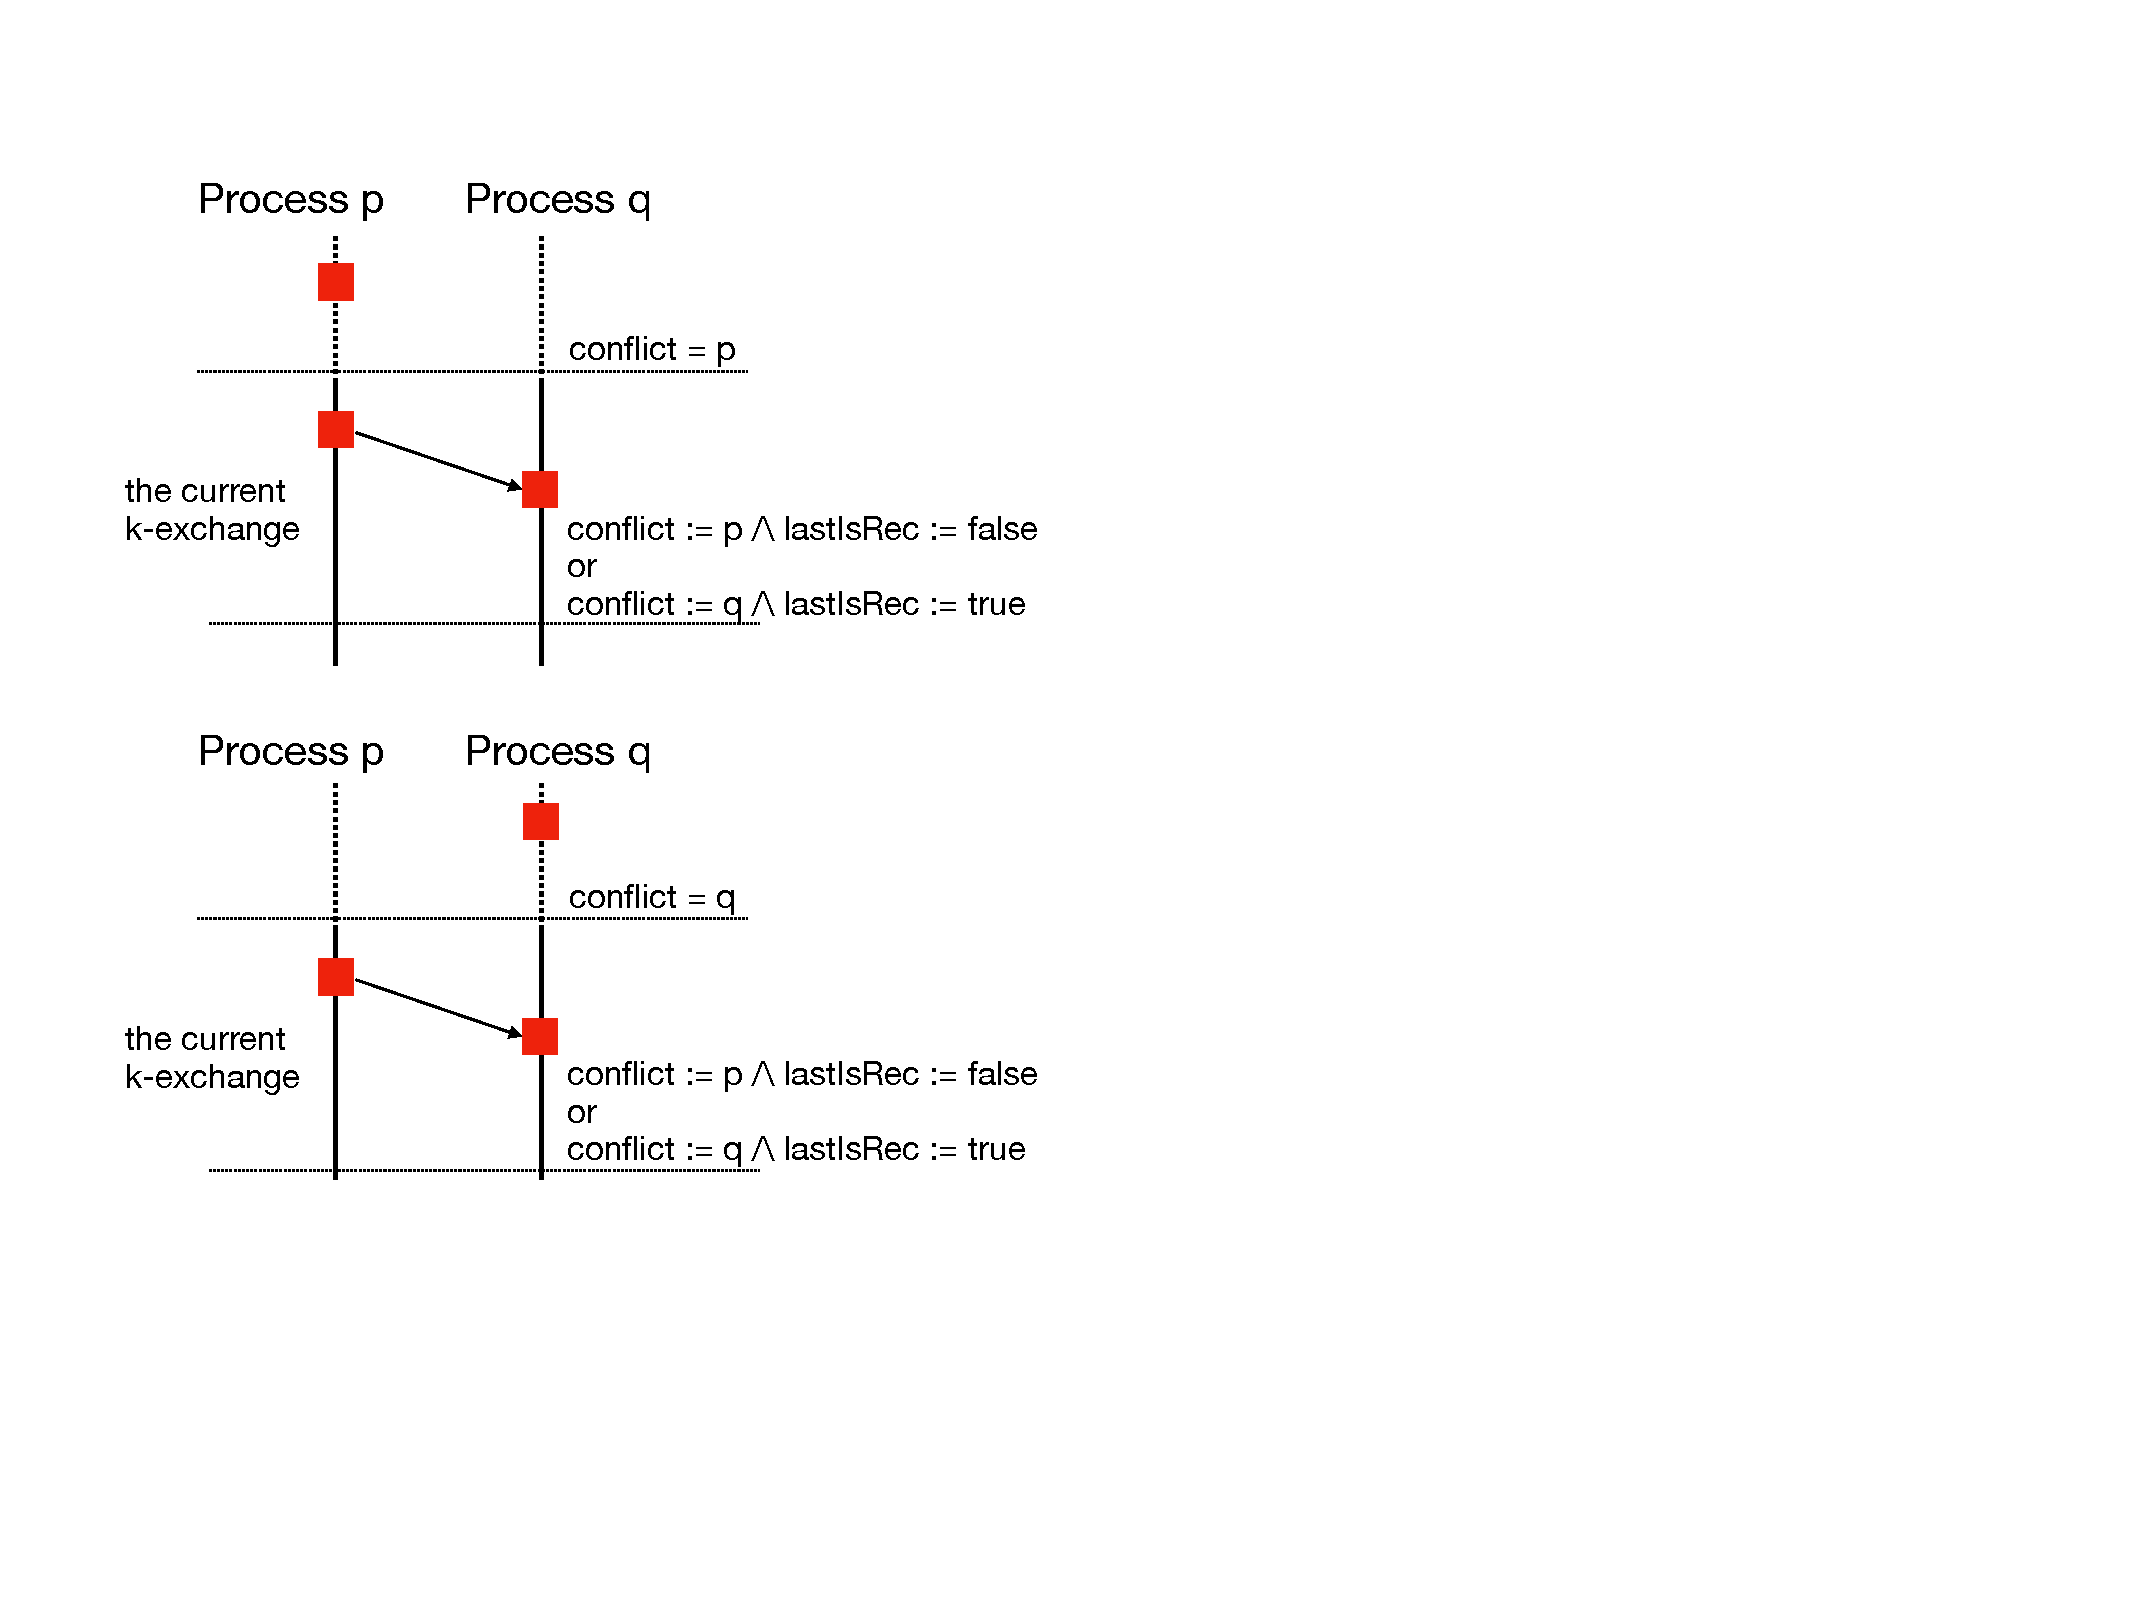
\includegraphics[width=5.5cm]{Borderline-mviol.pdf}
\end{minipage}
\caption{The monitor $\mathcal{M}_{\mathit{viol}}(k)$. We use $\mathbb{B}$ to denote the set of Boolean values and $\mathbb{N}$ the set of natural numbers. Initially, {\tt conflict} and {\tt receiver} are $\bot$, while {\tt lastIsRec} and {\tt sawRS} are {\tt false}.}
\label{fig:mon_viol}
\end{figure}

Figure~\ref{fig:mon_viol} lists the definition of $\mathcal{M}_{\mathit{viol}}(k)$ as an abstract state machine. Following the remarks above, when observing the send to $\pi$, the monitor updates the variable ${\tt conflict}$, which in general stores the process executing the last action in the cycle, to $p$. Also, a variable ${\tt count}$, which becomes $0$ when the cycle has strictly more than $k$ nodes, is initialized to $k$. 

Then, for every $k$-exchange transition in the execution, $\mathcal{M}_{\mathit{viol}}(k)$ non-deterministically picks pairs of matching send/receive or unmatched sends to continue the conflict-graph path, knowing that the last node represents an action of the process stored in ${\tt conflict}$. The rules for choosing pairs of matching send/receive to advance the conflict-graph path are pictured on the right of Figure~\ref{fig:mon_viol} (advancing the conflict-graph path with an unmatched send doesn't modify the value of ${\tt conflict}$, it just decrements the value of ${\tt count}$). In principle, there are two cases depending on whether the last node in the path conflicts with the send or the receive of the considered pair. One of the two process involved in this pair of send/receive equals the current value of ${\tt conflict}$. Therefore, ${\tt conflict}$ can either remain unchanged or change to the value of the other process. The variable {\tt lastIsRec} records whether the current conflict-graph path ends in a conflict due to a receive action. If it is the case, and the next conflict is between this receive and a send, then {\tt sawRS} is set to {\tt true} to record the fact that the path contains an $RS$ labeled edge (leading to a potential bad cycle).

When $\pi$ sends its message to $q$, the monitor checks whether the conflict-graph path it discovered ends in a node representing an action of $q$. If this is the case, this path together with the node representing the delayed send forms a cycle. Then, if ${\tt sawRS}$ is ${\tt true}$, then the cycle is bad and if ${\tt count}$ reached the value $0$, then the cycle contains more than $k$ nodes. In both cases, the current execution is a violation to $k$-synchronizability.

\section{Proofs of Section~\ref{sec:decidability}}\label{asec:decidability}

\begin{theorem}\label{th:dec1}
For a finite-state system $\mathcal{S}$, the reachability problem under the $k$-synchronous semantics is decidable and PSPACE-complete.
\end{theorem}
\begin{proof}
A consequence of the fact that the product emptiness problem (checking if the product of a set of finite state automata has an empty language) is PSPACE-complete~\cite{DBLP:conf/focs/Kozen77}. The evolution of the $B$ component of a synchronous configuration and the set of messages sent during a $k$-exchange transition can be modeled using an additional labeled transition system that is composed with the processes in the system. 
\end{proof}

\begin{theorem}
The problem of checking $k$-synchronizability of a finite-state system $\mathcal{S}$ is decidable and PSPACE-complete.
\end{theorem}
\begin{proof}
Theorem~\ref{th:main-verif} and Theorem~\ref{th:dec1} imply that the problem is in PSPACE. Moreover, PSPACE-hardness follows from the fact that the product emptiness problem can be reduced to checking $1$-synchronizability. Given a set of finite state automata $A_1$, $\ldots$, $A_n$, we define a message passing system $\mathcal{S}$ containing one process $p_i$ for each automaton $A_i$, which ``simulates'' the product. Essentially, $p_1$ is obtained from $A_1$ by rewriting every transition label $a$ to $\senda{p_1,p_2,a_1}\cdot \reca{p_1,a_n}$, the process $p_i$ with $1<i<n$ is obtained from $A_i$ by rewriting every transition label $a$ to $\reca{p_i,a_{i-1}}\cdot \senda{p_i,p_{i+1},a_i}$, and $p_n$ is obtained from $A_n$ by rewriting every transition label $a$ to $\reca{p_n,a_{n-1}}\cdot \senda{p_n,p_1,a_n}$. This rewriting ensures that every transition of the product of $A_1\times\ldots\times A_n$ is simulated precisely by a sequence of sends/receives:
\begin{align*}
\senda{p_1,p_2,a_1}\cdot \reca{p_2,a_1}\cdot \senda{p_2,p_3,a_2}\cdot\ldots \cdot \reca{p_n,a_{n-1}} \senda{p_n,p_1,a_n}\cdot \reca{p_1,a_n}
\end{align*}
Note that every execution admitted by this system is $1$-synchronous. Augmenting this system with new states and transitions to ensure that it produces a violation of $1$-synchronizability exactly when each process $p_i$ is in a final state of $A_i$, leads to a system which is \emph{not} $1$-synchronizable iff the product $A_1\times\ldots\times A_n$ has a non-empty language. Therefore, the product emptiness problem is polynomial-time reducible to checking $1$-synchronizability.
\end{proof}

\begin{theorem}
For a flow-bounded system $\mathcal{S}$, the problem of checking if there exists some $k$ such that $\mathcal{S}$ is $k$-synchronizable, is decidable.
\end{theorem}
\begin{proof}
First, assume that there exists an execution $e$ of $\mathcal{S}$ such that the corresponding conflict graph contains a bad cycle. Then, $\mathcal{S}$ is not $k$-synchronizable for $k = |e|$ (where $|e|$ denotes the length of $e$), and finding this $k$ through a procedure that checks $k$-synchronizability for increasing values of $k$ is clearly possible.

Now, assume that $\mathcal{S}$ admits no such execution. Then, every execution $e$ of $\mathcal{S}$ can be permuted to a $k$-synchronous execution $e'$, for some $k$ (the lack of conflict-graph cycles with an $RS$ labeled edge implies that the execution can be permuted to a sequence of $k$-exchange transition labels). Let $K$ be a constant such that every process in $\mathcal{S}$ is $K$-receive bounded and $K$-send bounded (this constant exists because $\mathcal{S}$ is flow-bounded). We get that the number of consecutive receives in $e'$ is bounded by $K\times |\<Pids>|$, and the number of consecutive sends by $K\times |\<Pids>|$. Otherwise, there would exist a process that performs more than $K$ consecutive receives or more than $K$ consecutive sends before a receive, which contradicts the definition of $K$. Therefore, $e'$ can be executed by a sequence of $K\times |\<Pids>|$-exchange transitions.
\end{proof}




\end{document}







